
\section{Experiment 1}
\label{sec:experiments}

In Experiment 1, we leveraged the Mouselab-MDP paradigm (Figure \ref{fig:MouselabMDP}) to evaluate how people plan against bounded-optimal planning and classic models of planning as search. 

%\fl{The structure of each experiment section models of planning.is
%\begin{enumerate}
%    \item We describe experiment-unique structure
%    \item We derive qualitative predictions.
%    \item Description of human data
%    \item Test of qualitative predictions
%    \item Test Quantitative model comparisons between the bounded-optimal strategy and previously proposed heuristics
%\end{enumerate}}
% Experiment 1: effect of increasing vs. decreasing variance
% Experiment 2: effect of low vs. high variance
% Experiment 3: branching and depth

\subsection{Methods}
\paragraph{Stimuli and Procedure}
\fl{TODO: Fred, Falk}

In the main part of the Each participant solved 30 different 3-step planning problems of the form shown in Figure \ref{fig:MouselabMDP}. There were 3 options for the first move and two options for the third move, leading to 6 paths in total. was independently drawn from a discrete uniform distribution over the values $-10,-5,+5$, and $+10$ and the cost of inspecting a node was \$$1$.

The main part of the experiment was proceeded by a series of practice blocks each of which explained one element of the task at a time and a quiz that queried participants about the range of rewards, the cost per click, and how their bonuses would be determined.

\paragraph{Participants: } We recruited $60$ participants from Amazon Mechanical Turk. Each participant received a base pay of $x$ and a performance dependent bonus of up to \$$x$ (average bonus: \$$y \pm z$). We excluded participants $9$ participants ($15$\%) because they either failed to follow the instruction to click during the training phase or answered less than 2 of the 3 comprehension checks correctly. 

\paragraph{Verbal protocol analysis}
\fl{TODO: Paul and Sayan}

\subsection{Models}

The probability $p(c|b,m)$ that a model $m$ assigns to performing computation $c$ in belief state $b$ is a weighted sum of two terms: 
\begin{dmath}
    p(c|b,m)=(1-p_{\text{random}})\cdot \sigma(c; V_{b,m}) + p_{\text{random}}\cdot \text{Uniform}(c; C_b).
\end{dmath}
The first part expresses its strategy's choice of computations as a soft-max function ($\sigma(c; V_{b,m})$) and the second part is an error model ($\text{Uniform}(c; C_b)$) according to which computations are chosen at uniformly at random from the set of available computations $C_b$ contains all clicks that have not been made yet and the termination action $\bot$. The weight $p_{\text{random}}$ of the error process is a free parameter that we constrain to be less than $0.25$. The strategy's preference 
\begin{equation}
\sigma(c; V_{b,m}) = \frac{ \exp( \frac{1}{\tau}\cdot V_{b,m}(c)) }{\sum_{c^\prime \in C_b} \exp( \frac{1}{\tau}\cdot V_{b,m}(c^\prime))},\label{eq:softMax}
\end{equation}
is determined by its preference function $V_{b,m}(c)$ and the decision temperature $\tau$.

\paragraph{Derivation and characterization of the bounded-optimal planning strategy}
%\fl{TODO: Fred and Falk}
We derived the bounded-optimal planning strategy by formulating the problem of deciding how to plan in Experiment 1 as a meta-level MDP and computing its optimal policy as described above.

We characterized the behavior of the bounded-optimal planning strategy by analyzing the probability $p(c|b,m_{\text{BO}})$ with which it chooses each planning operation for a series of 40 simulated trials. We discovered that the bounded-optimal strategy was similar to best-first search in that the nodes it inspects always lay on one of the inspectable paths with the highest expected return. However, it inspects those nodes in a different order than the classic best-first search algorithm and it makes distinct predictions about when people should terminate planning. Concretely, the bounded-optimal planning strategy makes the following predictions for Experiment 1:
predictions:
\begin{enumerate}
    \item  The first observed node is a stem or branch node rather than a leaf node.
    \item Participants make at least two clicks on every trial.
    \item If the first observed value is above average, people should stay on the same branch, else they should switch to a different branch.
    \item If the first observed node is a non-leaf and its revealed value is positive but small (+5), then people should inspect another non-leaf on the same branch, and if its revealed value is large and positive (+10), then people should inspect a leaf on the same branch.
    \item People should always inspect a node that lies on a path with maximal expected return.
    \item Once a branch with at least one uninspected leaf has an expected return at least 10 points larger than any other branch people should skip to inspecting its leafs even if it has uninspected branch or stem nodes.
    \item The satisficing level starts out very high ($>20$ after 1 click and 20 after two clicks) and then decays as additional clicks are made (10 after 3 clicks, -5 after 11 clicks). Therefore, the smallest expected reward with which a person stops should be decreasing with the number of clicks.
\end{enumerate}


\paragraph{Models of classical planning strategies}
%\fl{TODO: Priyam}
In order to evaluate our bounded-optimal planning strategy against previously proposed planning strategies, we built likelihood models of the classical planning strategies known as depth first search, breadth first search, and best first search. We also built a likelihood model of a strategy proposed by \citet{NewellSimon1972a}, called simple progressive deepening search. Each strategy $m$ was defined in terms of the values $V_{b,m}(c)$ it assigns to the different clicks $c$ depending on the current belief state $b$ (see Equation \ref{eq:softMax}). The preference functions were defined as follows:
\begin{itemize}
    \item \textit{Depth First Search:} This function prioritizes deeper nodes on partially observed paths by assigning higher values to $c$ for deeper nodes. 
    \item \textit{Breadth First Search:} This function prioritizes shallower nodes on partially observed paths. 
    \item \textit{Best First Search:} This function prioritizes nodes on promising paths by assigning the expected value of rewards along the path on which $c$ lies to $c$. Best First also considers clicks on a path in sequential order. 
    \item \textit{Simple Progressive Deepening Search:} This function prioritized deeper nodes similarly to Depth First search. However, once a path is fully explored, the starting nodes of any sub-paths that may branch off from it receive the same value as the starting nodes of other, separate paths.
\end{itemize}
Clicks that are inconsistent with the given strategy $m$ are assigned very small values. Our models also included a threshold for satisficing \cite{Simon1956} and a threshold for pruning \cite{Huys2012}. When $c = \bot$, the expected reward for terminating in the current state $b$ is compared to the satisficing threshold. If the expected reward equals or exceeds the satisficing threshold, then all preference functions return a very large value so that the terminating action gets the highest preference. For pruning, the total expected reward of path along which $c$ lies is compared to the pruning threshold. If the expected reward does not exceed the pruning threshold, $c$ receives a value such that all other clicks are considered before those on the pruned path. Both the checks for satisficing and pruning occur before the rest of the strategy specific preference function executes.
%\pd{Suggestions are warmly welcomed.} %\fl{I have described the softmax component and error model above as it is shared between all models. Please add a description of each model's preference function and a description of satisficing and pruning.} 



\paragraph{Directed cognition model}
\fl{TODO: Sayan}


\subsection{Results}

%When people clicked there clicks were bounded-optimal about 61.2\% of the time.

\paragraph{Model Comparisons}
\fl{TODO: Fred and Priyam}



\paragraph{Qualitative predictions}
We found that our participants' planning strategies conformed to the first three predictions. Consistent with prediction 1, the majority of participants' first clicks were significantly more often directed at stem or branch nodes than at leaf nodes ($82.6\%$ vs. $17.4\%$, $p<10^{-15}$) even though there are just as many leaf nodes as branch and stem nodes combined. However, unlike the bounded-optimal strategy, people preferred stem nodes over branch nodes ($72.6\%$ vs. $10.0\%$, $p<10^{-15}$). Consistent with prediction 2, participants inspected at least two nodes on $89.1\%$ of the trials. Consistent with prediction 3, participants usually switched the branch if the observed value was below average ($86.4\%$ of the time, $p=1.787894216482486e-57$), but stayed on the same branch if the observed value was above average ($59.7\%$ of the time, $p=.00001$).
However, participants planning strategies violated both parts of prediction 4 more than half of the time. Following a large positive observation at the beginning of a branch, participants inspected a leaf of that branch only $28.9\%$ of the time; instead they inspected the other non-leaf of that branch $51.5\%$ of the time. Following a small positive reward they inspected another non-leaf node on the same branch only $25.1\%$ of the time; instead they switched to another branch $57.0\%$ of the time.
Consistent with prediction 5, participants' clicks gathered information about one of the most promising paths $82.1\%$ of the time ($p<10^{-15}$). Consistent with prediction 6, when a branch with at least one uninspected leaf had an expected return that was at least 10 points larger than the expected return of any other branch people start inspecting its leafs $79.6\%$ of the time.
To test the last prediction, we estimated people's aspiration level as a function of their number of clicks by the lower quartile of their expected return when they stopped clicking. While this estimate of their aspiration level was negatively correlated with the number of clicks (Spearman's $\rho=-0.29$) this effect was not statistically significant ($p=0.38$).

\paragraph{Quantifying deviations from bounded optimality.}  We found that, on average, $45.0\%$ of our participant's computations were sub-optimal. However, the computations people selected did nevertheless achieve $86.8\%$ of the highest possible value of computation ($\text{VOC}(b,c)=Q\meta^\star(b,c) - Q\meta^\star(b,\bot)$).
Next, we characterized in which ways people's planning strategies are sub-optimal. We found that people tend to plan too little. Concretely, $28.3\%$ of the time people deviate from optimal planning it is  because they terminate too early, whereas it occurred only $6.3\%$ of the time that people continued planning when it would have been bounded-optimal to stop. Finally, the majority of people's deviations from bounded optimality (i.e., $65.5\%$) occurred when people clicked on one node whereas the bounded optimal strategy would have clicked on a different node. 

In summary, we found three systematic deviations from bounded-optimal planning: People preferred to inspect equally informative nodes sequentially starting from the beginning but bounded-optimal planning does not. Second, people tend to stop planning too early. Third, following a (very) good observation on the first click, people continue to explore broadly whereas bounded-optimal planning would already focus the second click on the promising paths identified by that observation.

\paragraph{Individual differences in rationality.} Consistent with previous work by \cite{Stanovich1998} we found considerable inter-individual differences in the extent to which people's planning strategies were rational (see Figure \ref{fig:individual-differences}). The average agreement between people's planning operations and bounded-optimal planning ranged from $0\%$ to $80.8\%$ (average $48.0\%$, standard deviation $23.3\%$); and the average VOC of people's planning operations ranged from $0$\% to $98.5$\% of the optimal VOC (mean $80.0$\%, standard deviation $26.4$\%). Interestingly, Figure \ref{fig:individual-differences}b suggests that the majority of participants used planning strategies that achieve a high level of resource-rationality and that the frequency of alternative strategies decrease with the degree to which they were suboptimal, and Figure \ref{fig:individual-differences}a suggested that the distribution of people's rationality scores might be bimodal.

\begin{figure}
a)

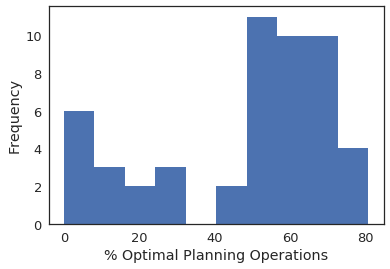
\includegraphics[width=0.48\textwidth]{figures/optimal-planning-operations.png}

b)

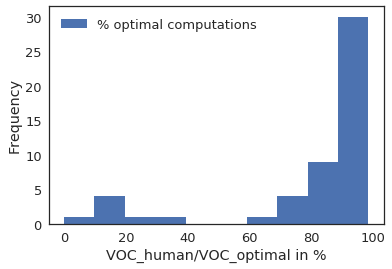
\includegraphics[width=0.48\textwidth]{figures/VOC-ratio.png}
\caption{Individual differences in the rationality of people's planning strategies.}
\label{fig:individual-differences}
\end{figure}


\paragraph{Verbal protocol analysis}
\fl{TODO: Paul and Sayan}

\section{Experiment 2: Adaptation to the structure of the environment}

Bounded optimality predicts that people should adapt their planning strategies to the structure of the environment. Here, we test this prediction by manipulating whether future rewards are more variable than immediate rewards or vice versa.

\subsection{Methods}
Experiment 2 presented participants with a modified version of the three-step planning problem used in Experiment 1 (see Figure \ref{fig:MouselabMDP}). Each participant was randomly assigned to one of two conditions. The critical difference between these conditions was that the variability of the reward distribution either increased or decreased with the number of steps it takes to reach a node. Concretely, in the first condition the reward distributions were $\text{Uniform}(\lbrace -4,-2,+2,+4 \rbrace)$, $\text{Uniform}(\lbrace -8,-4,+4,+8 \rbrace)$, and $\text{Uniform}(\lbrace -48,-24,+24,+48 \rbrace)$ for nodes reachable in one, two, and three steps respectively. In the second condition, the order of these three outcome distributions was reversed. The instructions informed participants about this reward structure and they further received 10 practice trials with fully revealed reward structures in which they could learn the statistics of the environment from experience.

%Each participant was randomly assigned to one of three conditions: The first condition was identical to Experiment 1. In the second condition the variability of the reward distribution was scaled down by a factor of 10 (($\sigma_R=1$)). In the third condition the variability $\sigma_R$ of the rewards increased outwardly from $X$ in the first step, to $Y$ in the second step, and $Z$ in the third step.

We computed the bounded-optimal planning strategy for each environment and characterized its behavior.%of the three environments using the meta-level reinforcement learning algorithm developed by \cite{LiederCallawayGulKruegerGriffiths2017}. We characterized the behavior of the three resulting planning strategies to derive the predictions presented below.

\fl{TODO: Falk and Fred}

\subsection{Results}

\paragraph{Model predictions}
Bounded optimality predicted that people should use qualitatively different planning strategies in these two environments. Broadly speaking, when the variance of the reward distribution increases with the number of steps then people should plan backward from potential end states. By contrast, when the variance decreases with each step, then people should plan forward from their initial state. To be concrete, the bounded optimal planning strategy for the environment with increasing variance predicts that participants in Condition 1 should ...
\begin{enumerate}
    \item always make their first click on a potential end state
    \item never inspect a non-leaf before all leafs have been inspected
    \item immediately stop planning when they discover that one of the end states yields the largest possible reward
    \item only inspect the reward of the first step or second step if there is a tie between the rewards of the best end states
    \item start resolving such ties by inspecting the second-step rewards of one of the best paths
\end{enumerate}
By contrast, the bounded optimal planning strategy for the environment with decreasing variance predicts that participants in Condition 2 should
\begin{enumerate}
    \item use their first click to inquire about one of the immediate rewards
    \item continue to inspect immediate rewards with their second click unless the first click revealed the largest possible reward
    \item make their second click on one of the end states if their first click reveals the largest possible reward
\end{enumerate}

\paragraph{Human performance}

We found that ...
\fl{TODO: Fred, Falk, and Priyam}

Verbal protocol analysis revealed that ...
\fl{TODO: Paul and Sayan}

\paragraph{Planning focuses on the most informative outcomes}
Bounded optimality predicts that people's planning strategy should prioritize state-action pairs that might yield large positive or large negative outcomes over state-action pairs whose rewards will be rather negligible. Concretely, since the variance of the reward distribution in Condition 3 increases outwardly, bounded optimality predicts that participants in Condition 3 should start by inspecting the possible end-states until they find one that is good enough and only resort to inspecting the more immediate rewards if the two best possible end-states are identical.

We found that ...
\fl{TODO: Fred, Falk, and Priyam}



Verbal protocol analysis revealed that ...
\fl{TODO: Paul and Sayan}

%\subsection{Experiment 2: low vs. high variability}
%\fl{Here, the basic prediction is that higher variability in the reward distribution favors more planning.}
%\subsection{Experiment 2: increasing vs. decreasing variability}
%\fl{Here, the basic prediction is that backward planning is optimal when the variability in the achievable reward increases into future than when it decreases.}
%\subsection{Experiment 3: branching and depth}